%% LaTeX Beamer presentation template (requires beamer package)
%% see http://bitbucket.org/rivanvx/beamer/wiki/Home
%% idea contributed by H. Turgut Uyar
%% template based on a template by Till Tantau
%% this template is still evolving - it might differ in future releases!

\documentclass{beamer}

\mode<presentation>
{
\usetheme{Warsaw}

\setbeamercovered{transparent}
}

\usepackage[english]{babel}
\usepackage[latin1]{inputenc}

% font definitions, try \usepackage{ae} instead of the following
% three lines if you don't like this look
\usepackage{mathptmx}
\usepackage[scaled=.90]{helvet}
\usepackage{courier}

\usepackage[T1]{fontenc}

% User packages
\usepackage[absolute,overlay]{textpos}
\usepackage{tikz}
\usepackage{listings}

\title{Birdhouse - supporting Web Processing Services}

%\subtitle{}

% - Use the \inst{?} command only if the authors have different
%   affiliation.
\author{\vspace{2.3cm}\\
Carsten Ehbrecht\inst{1}
\and Stephan Kindermann\inst{1}
\and Nils Hempelmann\inst{2}
}
%\author{\inst{1}}

% - Use the \inst command only if there are several affiliations.
% - Keep it simple, no one is interested in your street address.
\institute[Institute]
{
\inst{1}%
DKRZ - German Climate Compute Center
\and
\inst{2}%
GIZ - German Development Cooperation
}

\date{\footnotesize{$28^{th}$ of November 2017/ Python Frameworks Workshop at ECMWF}}


% This is only inserted into the PDF information catalog. Can be left
% out.
\subject{Talks}



% If you have a file called "university-logo-filename.xxx", where xxx
% is a graphic format that can be processed by latex or pdflatex,
% resp., then you can add a logo as follows:

% \pgfdeclareimage[height=0.5cm]{university-logo}{university-logo-filename}
% \logo{\pgfuseimage{university-logo}}



% Delete this, if you do not want the table of contents to pop up at
% the beginning of each subsection:
\AtBeginSubsection[]
{
\begin{frame}<beamer>
\frametitle{Outline}
\tableofcontents[currentsection,currentsubsection]
\end{frame}
}

% Section title slides
\AtBeginSection[]{
  \begin{frame}
  \vfill
  \centering
  \begin{beamercolorbox}[sep=8pt,center,shadow=true,rounded=true]{title}
    \usebeamerfont{title}\insertsectionhead\par%
  \end{beamercolorbox}
  \vfill
  \end{frame}
}


% If you wish to uncover everything in a step-wise fashion, uncomment
% the following command:

%\beamerdefaultoverlayspecification{<+->}

\begin{document}

\begin{frame}
   % \tikz [remember picture,overlay]
   %  \node at
   %      ([yshift=4.8cm]current page.south)
   %      %or: (current page.center)
   %      {
\includegraphics[height=2.8cm]{images/pywps}};
   \titlepage
\end{frame}

\begin{frame}
\frametitle{Outline}
\tableofcontents
% You might wish to add the option [pausesections]
\end{frame}

% %%%%%%%%%%%%%%%%%%%%%%%%%%%%%%%%%%%%%%%%%%%%%%%%%%%%%%%%%%%%%%%%%%%%%%%%%%%%%
\section{Motivation}

%\subsection[Short First Subsection Name]{First Subsection Name}


% -----------------------------------------------
\begin{frame}
\frametitle<presentation>{The OGC Web Processing Service}

  \begin{figure}[ht]

   \centering
   
\includegraphics[height=5cm]{images/WPS}
  \end{figure}

\centering
\footnotesize{\url{http://www.slideshare.net/TheodorFoerster/restful-web-processing-service}}

\end{frame}

% -----------------------------------------------
\begin{frame}
\frametitle<presentation>{WPS Use Case}

  \begin{figure}[ht]
    \centering
    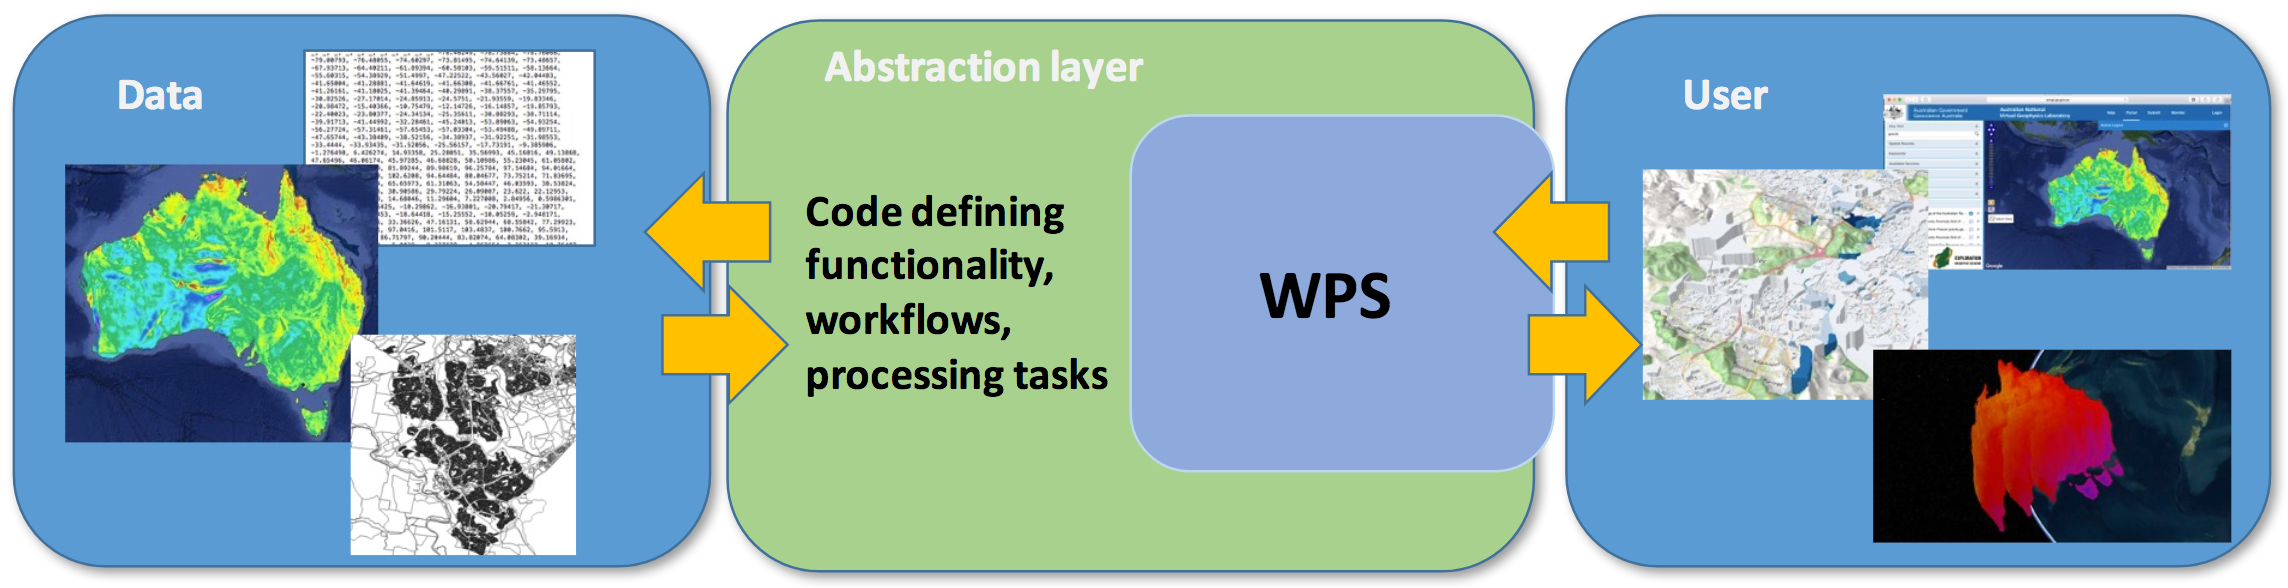
\includegraphics[width=11.5cm]{images/wps_adamsteer}
  \end{figure}

\centering
\footnotesize{WPS for Point Clouds by Adam Steer, NCI, Australia}

\end{frame}

% -----------------------------------------------
\begin{frame}
\frametitle<presentation>{WPS Inputs and Outputs}

  \begin{figure}[ht]
    \centering
    \includegraphics[width=11.5cm]{images/wps-ensemble-robustness}
  \end{figure}

  %\centering
  %\footnotesize{Statistical analysis of climate model data}

\end{frame}

% -----------------------------------------------
\begin{frame}[fragile]
  \frametitle<presentation>{Function as a Service}
    \lstset{language=python} \lstinputlisting{static/wps_myplot.py}
\end{frame}

% -----------------------------------------------
\begin{frame}[fragile]
  \frametitle<presentation>{Running Function as Web Processing Service}
    \begin{verbatim}
$ curl -s -o result.xml \
http://localhost/wps? \
 &service=WPS \
 &version=1.0.0 \
 &request=execute \
 &identifier=myplot \
 &DataInputs=nc_file=http://;variable=tas
    \end{verbatim}
\end{frame}

% %%%%%%%%%%%%%%%%%%%%%%%%%%%%%%%%%%%%%%%%%%%%%%%%%%%%%%%%%%%%%%%%%%%%%%%%%%%%%
\section{PyWPS}

% -----------------------------------------------
\begin{frame}
\frametitle<presentation>{What is PyWPS?}

\begin{figure}[ht]
  \centering
  
\includegraphics[height=2cm]{images/pywps}
\end{figure}

\begin{itemize}
  \item An implementation of the OGC Web Processing Service standard
  \item Implements WPS 1.0.0 standard (WPS 2.0.0 in progress)
  \item Coded in the Python language (researcher friendly)
  \item Easy to hack (developer friendly)
  \item Relevant contributions by over a dozen individuals
  \item OSGeo accreditation around the corner \ldots
\end{itemize}

\vspace{0.2cm}
\centering
\footnotesize{\url{http://pywps.org}}

\end{frame}


% -----------------------------------------------
\begin{frame}
\frametitle<presentation>{The WSGI Onion}

\begin{tikzpicture}[remember picture,overlay]
    \node[xshift=-9.2cm,yshift=-5.8cm] at (current page.north east)
    {
\includegraphics[height=6cm]{images/wsgi-onion}};
\end{tikzpicture}

\begin{textblock*}{5cm}(7cm,4cm)
\begin{itemize}
  \item Nginx - security, reverse proxy, load balancing
  \item Gunicorn - concurrency, WSGI
  \item WSGI App - PyWPS WSGI application
\end{itemize}
\end{textblock*}
\end{frame}


% -----------------------------------------------
\begin{frame}
\frametitle<presentation>{It's complicated!}

\begin{itemize}

  \item Scalability requires the orchestration of various software layers:
   \begin{itemize}
	  \item Nginx
	  \item Gunicorn
	  \item PyWPS
	\end{itemize}
  \item Many packages to install
  \item Many configurations to set-up
  \item No clients for testing
\end{itemize}

\vspace{0.4cm}
\centering
\Large{Too much work?}

\end{frame}


% %%%%%%%%%%%%%%%%%%%%%%%%%%%%%%%%%%%%%%%%%%%%%%%%%%%%%%%%%%%%%%%%%%%%%%%%%%%%%
\section{Birdhouse}

% -----------------------------------------------
\begin{frame}
\frametitle<presentation>{What is Birdhouse?}

\begin{itemize}
  \item Supporting OGC Web Processing Services in the climate science community.
  \item Making it easier to set-up WPS services (Birdhouse-Builder).
  \item Providing Python library and WPS processes to access climate data.
  %\item Providing a workflow to chain data fetching and data processing.
  \item Providing a security proxy middleware to protect OGC/WPS services.
  \item Providing a web application and command-line client to interact with WPS services.
  \item \url{http://bird-house.github.io/}

\end{itemize}
\end{frame}


% -----------------------------------------------
\begin{frame}
\frametitle<presentation>{Birdhouse Overview}

  \begin{figure}[ht]
    \centering
    \includegraphics[height=5.85cm]{images/birdhouse-overview}
  \end{figure}

\end{frame}

% -----------------------------------------------
\begin{frame}
\frametitle<presentation>{WSGI Application controlled by Supervisor}

  \begin{figure}[ht]
    \centering
    \includegraphics[height=7cm]{images/wsgi-app}
  \end{figure}

\end{frame}

% -----------------------------------------------
\begin{frame}
  \frametitle<presentation>{Manage the Chaos}

  \begin{tikzpicture}[remember picture,overlay]
      \node[xshift=-9.5cm,yshift=-5cm] at (current page.north east)
      {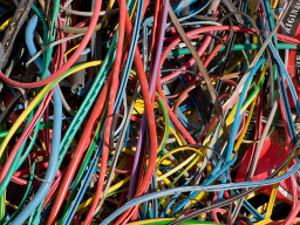
\includegraphics[height=3.5cm]{images/chaos}};
  \end{tikzpicture}

  \begin{textblock*}{7cm}(6cm,3cm)
  \begin{itemize}
    \item Many components: PyWPS, Nginx, Gunicorn, ncWMS, \ldots
    \item Lots of packages: cdo, cfchecker, OCGIS, numpy, R, ESMValTool, \ldots
    \item Many configurations to set-up
    \item Reproducible installation
    \item Different Linux distributions (Centos, Debian, \ldots)
  \end{itemize}
  \end{textblock*}
\end{frame}

% -----------------------------------------------
\begin{frame}[fragile]
  \frametitle<presentation>{Conda Package Manager}
  \begin{itemize}
    \item Originally for python ... but has a general concept
    \item Does not need admin rights
  \end{itemize}
  Install PyWPS from birdhouse channel
    \begin{verbatim}
$ conda install -c birdhouse pywps
    \end{verbatim}
  Create conda environment \textbf{pywps}
    \begin{verbatim}
$ conda create -n pywps -c birdhouse pywps
    \end{verbatim}
\end{frame}

% -----------------------------------------------
\begin{frame}[fragile]
  \frametitle<presentation>{Deployment with Buildout}
  \begin{itemize}
    \item Makefile to wrap Buildout commands
    \item A common deployment pattern for all Birds
  \end{itemize}
    \begin{verbatim}
$ git clone https://github.com/bird-house/emu.git
$ cd emu
$ make clean install
$ make start
    \end{verbatim}
  Update configuration like hostname, port
    \begin{verbatim}
$ vim custom.cfg
$ make update
$ make restart
    \end{verbatim}
\end{frame}

% -----------------------------------------------
\begin{frame}
\frametitle<presentation>{Docker}

\begin{itemize}
  \item Docker Hub is a public repository for dockerfiles
  \item Birdhouse repository with automatically updated docker images
\end{itemize}

  \begin{figure}[ht]
   \centering
   \includegraphics[height=3.6cm]{images/dockerhub.png}
  \end{figure}

\vspace{0.2cm}
\centering
\footnotesize{\url{https://hub.docker.com/u/birdhouse/}}

\end{frame}

% -----------------------------------------------
\begin{frame}[fragile,shrink]
  \frametitle<presentation>{Try a Docker \ldots}

  \begin{tikzpicture}[remember picture,overlay]
      \node[xshift=-3cm,yshift=-7cm] at (current page.north east)
      {\includegraphics[height=3cm]{images/docker}};
  \end{tikzpicture}

  Running a docker image with Emu WPS on port 8080
    \begin{verbatim}
$ docker pull birdhouse/emu
$ docker run -it -p 8000:8000 -p 8080:8080 \
       --name=emu_wps birdhouse/emu
    \end{verbatim}
  Running a WPS GetCapabilities request
    \begin{verbatim}
$ curl -s -o caps.xml \
http://localhost:8080/wps? \
  service=WPS& \
  version=1.0.0& \
  request=GetCapabilities
    \end{verbatim}
\end{frame}

% -----------------------------------------------
\begin{frame}
  \frametitle<presentation>{Phoenix web-based WPS client}
  \begin{figure}[ht]
    \centering
    \includegraphics[width=10cm]{images/phoenix}
  \end{figure}
\end{frame}

% -----------------------------------------------
\begin{frame}
  \frametitle<presentation>{Phoenix Example}
  \begin{figure}[ht]
    \centering
    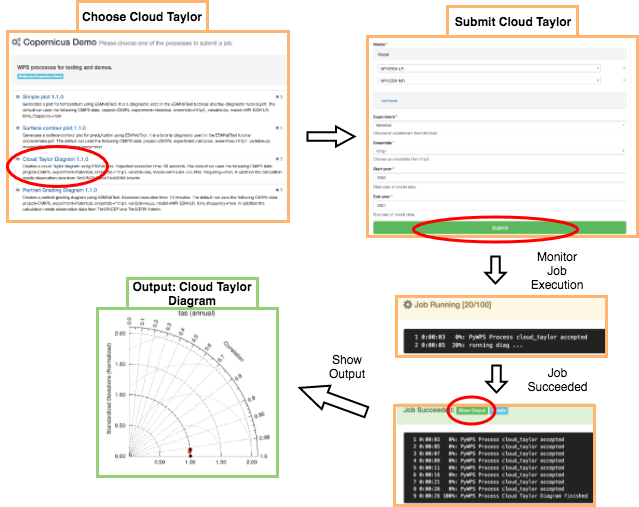
\includegraphics[height=6cm]{images/phoenix-example}
  \end{figure}
\end{frame}

% -----------------------------------------------
\begin{frame}[fragile]
  \frametitle<presentation>{Birdy command line WPS client}
  \begin{verbatim}
$ conda install -c birdhouse birdhouse-birdy
$ export WPS_SERVICS=http://localhost:8094/wps
$ birdy -h
  \end{verbatim}
  \begin{figure}[ht]
    \centering
    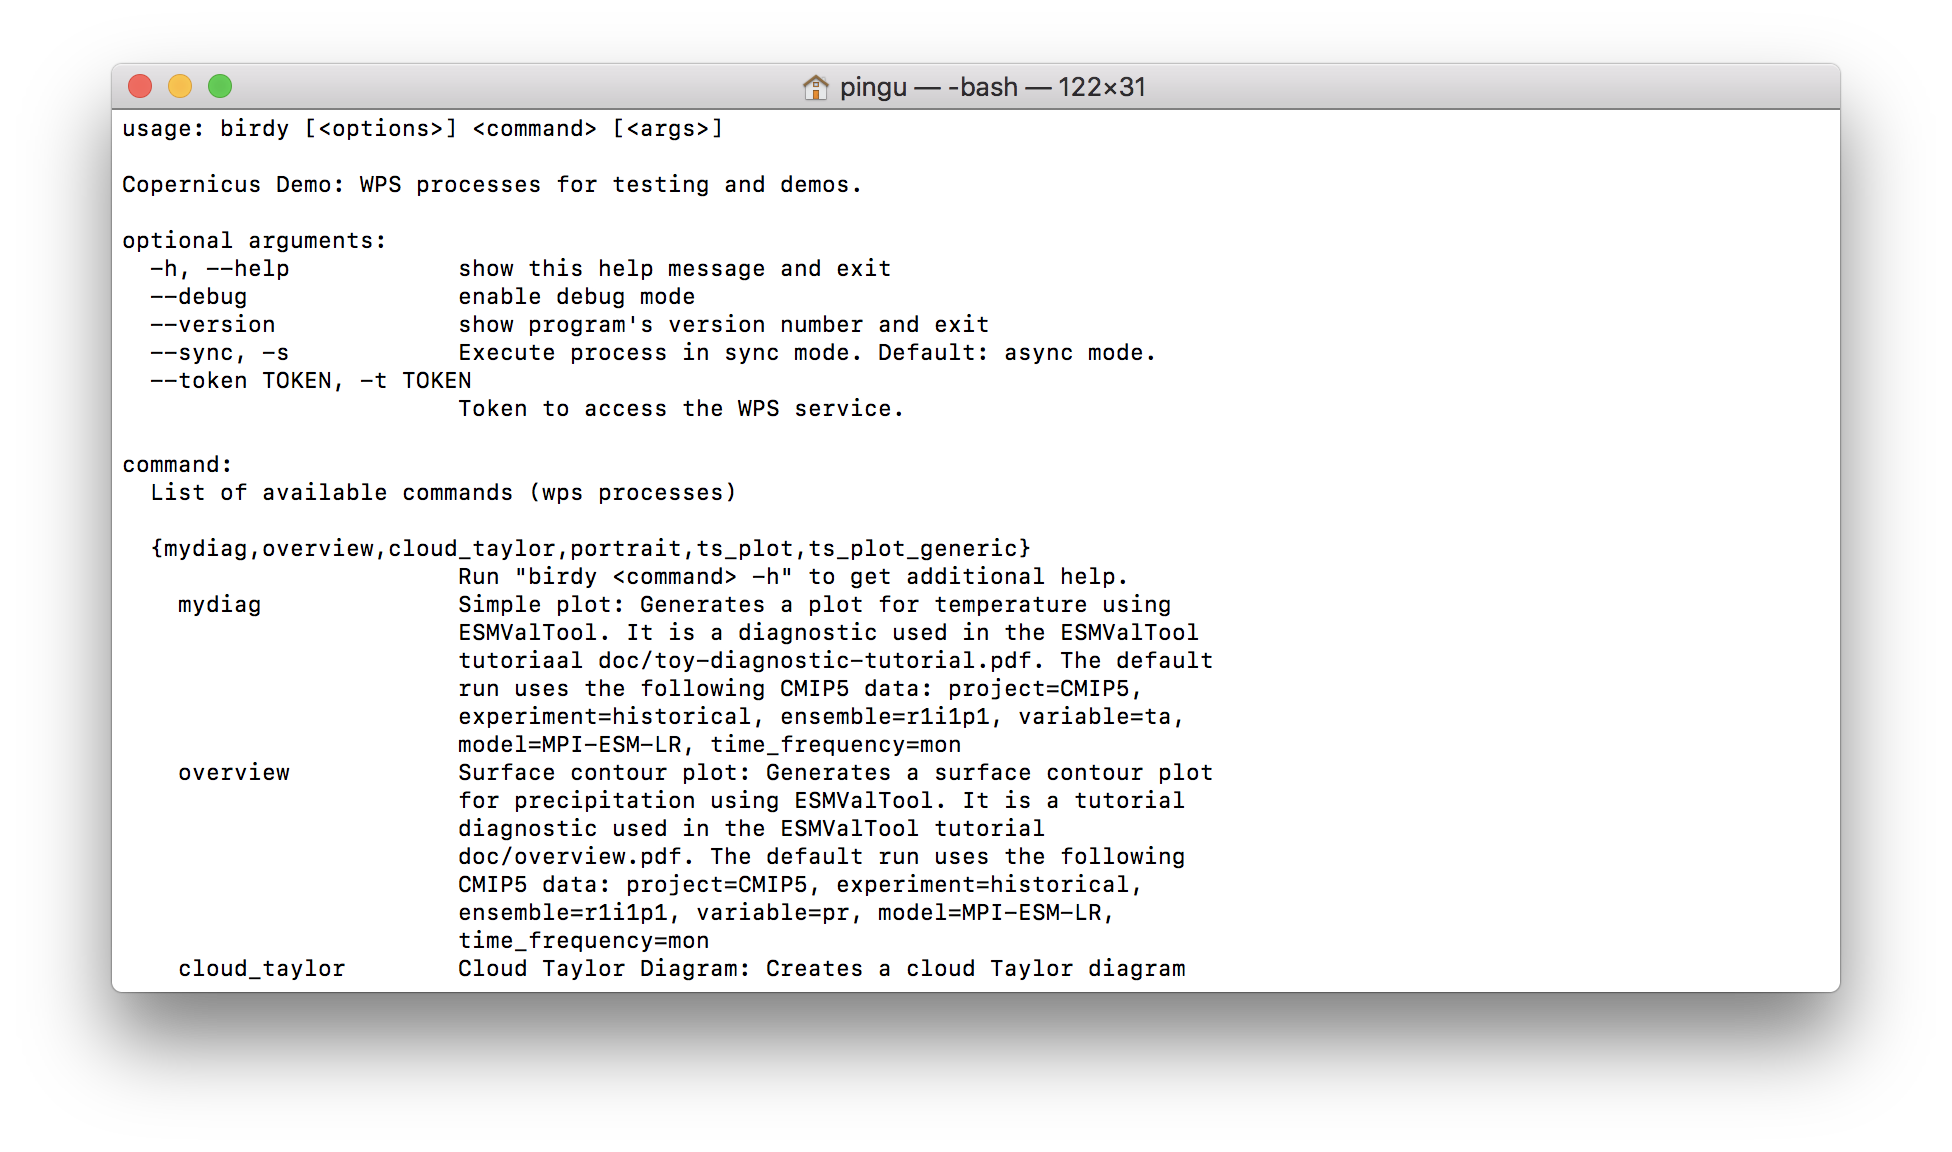
\includegraphics[height=4cm]{images/birdy-terminal}
  \end{figure}
\end{frame}

% -----------------------------------------------
\begin{frame}
  \frametitle{WPS Security Proxy}
  \begin{itemize}
    \item Using string token (uuid) as part of URL or in request header to protect WPS execute access
    \item X509 certificates to access (remote) data from ESGF are provided by proxy (using environ)
    \item Implemented as WSGI middleware service
    \item \url{http://twitcher.readthedocs.io/en/latest/}
  \end{itemize}
  \begin{figure}
    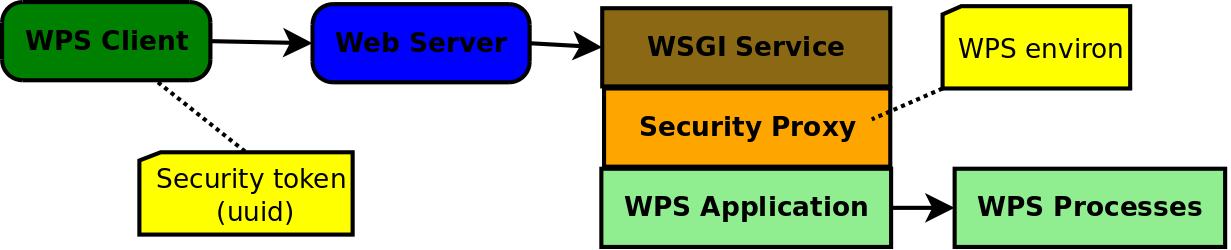
\includegraphics[width=11.0cm]{images/wps-proxy}
  \end{figure}
\end{frame}

% %%%%%%%%%%%%%%%%%%%%%%%%%%%%%%%%%%%%%%%%%%%%%%%%%%%%%%%%%%%%%%%%%%%%%%%%%%%%%
\section{Projects}

% -----------------------------------------------
\begin{frame}
\frametitle<presentation>{Copernicus: ESMValTool diagnostics as WPS}

  \begin{figure}[ht]
    \centering
    \includegraphics[height=5cm]{images/copernicus-wps}
  \end{figure}

  \centering
  \footnotesize{\url{https://www.esmvaltool.org/}}

\end{frame}

% -----------------------------------------------
\begin{frame}
\frametitle<presentation>{Copernicus: Example Run}

  \begin{figure}[ht]
    \centering
    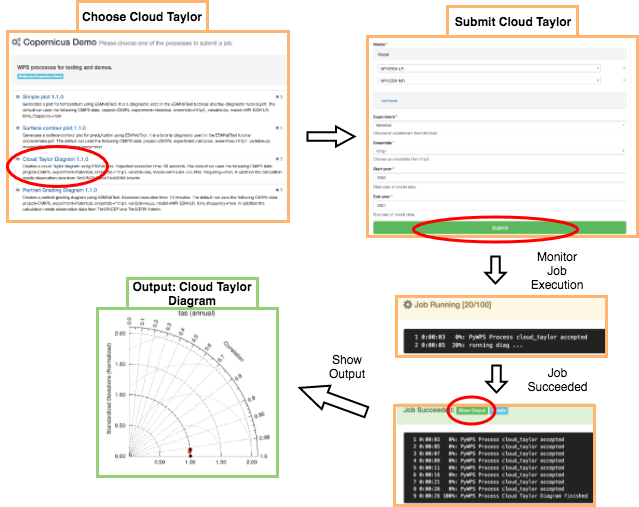
\includegraphics[height=5cm]{images/phoenix-example}
  \end{figure}

  \centering
  \footnotesize{\url{https://bovec.dkrz.de/processes/list?wps=copernicus}}

\end{frame}

% -----------------------------------------------
\begin{frame}
\frametitle<presentation>{Copernicus: PyWPS Scheduler Extension}

  \begin{figure}[ht]
    \centering
    \includegraphics[width=11.5cm]{images/pywps-scheduler-extension}
  \end{figure}

  \centering
  \footnotesize{This extension is part of PyWPS}

\end{frame}

% -----------------------------------------------
\begin{frame}
  \frametitle{PAVICS: A Platform for the Analysis and Visualization of Climate Science}

  \begin{tikzpicture}[remember picture,overlay]
      \node[xshift=-10cm,yshift=-5cm] at (current page.north east)
      {\includegraphics[width=5cm]{images/pavics}};
  \end{tikzpicture}

  \begin{textblock*}{7cm}(5cm,3cm)
  \begin{itemize}
    \item Project based on Birdhouse by Ouranos and CRIM, Canada
    \item Ouranos needs a platform for climate services
    \item Creating and delivering climate products
    \item Make climate research less painful
  \end{itemize}
  \end{textblock*}

  \vspace{3cm}
  \centering
  \footnotesize{\url{https://www.researchgate.net/project/PAVICS}}
\end{frame}


% %%%%%%%%%%%%%%%%%%%%%%%%%%%%%%%%%%%%%%%%%%%%%%%%%%%%%%%%%%%%%%%%%%%%%%%%%%%%%
\section{Summary}

\begin{frame}
\frametitle<presentation>{Summary}

\begin{itemize}

  \item Deployment
  \begin{itemize}
    \item Nginx + Gunicorn provide the infrastructure for scalable services
    \item Birdhouse supports automatic deployment using Conda and Buildout
  \end{itemize}

  \item{Toolbox}
  \begin{itemize}
    \item Web portal and command-line tool for testing and demo of WPS services
    \item Security middleware to protect the execution of WPS processes
  \end{itemize}

  \item{Get your hands dirty}
  \begin{itemize}
    \item Birdhouse Workshop: \url{http://birdhouse-workshop.readthedocs.io/en/latest/index.html}
    \item PyWPS Workshop: \url{https://github.com/PyWPS/pywps-workshop}
  \end{itemize}
\end{itemize}

\end{frame}

% --------------------------------------------------------------
\begin{frame}
%\frametitle<presentation>{}

  \begin{figure}[ht]
   \centering
   \includegraphics[height=4.5cm]{images/for_the_birds}
  \end{figure}

\centering
\Huge{The End}

\centering
\vspace{0.4cm}
\footnotesize{\url{http://bird-house.github.io/}}
\end{frame}

% %%%%%%%%%%%%%%%%%%%%%%%%%%%%%%%%%%%%%%%%%%%%%%%%%%%%%%%%%%%%%%%%%%%%%%%%%%%%%
\appendix

\section{Appendix}

% -----------------------------------------------
\begin{frame}
\frametitle<presentation>{The OGC Web Processing Service}

\begin{itemize}
\item OGC open web standard for remote geo-spatial processing.
\item Other widley used OGC web standards: \textbf{WMS}, \textbf{WFS}, \textbf{WCS}.
\item Three basic requests:
\begin{itemize}
      \item  \textit{GetCapabilities}
      \item  \textit{DescribeProcess}
      \item  \textit{Execute}
\end{itemize}
\item Three basic input/output classes:
\begin{itemize}
      \item  \textit{Literal}
      \item  \textit{Complex} - for geo-spatial data and services
      \item  \textit{BoundingBox} - for geo-spatial data extent
\end{itemize}
\end{itemize}
\end{frame}

% -----------------------------------------------
\begin{frame}
  \frametitle<presentation>{What does WPS provide?}
  \begin{itemize}
    \item web access to your algorithms (GET request with key-value, POST request with xml)
    \item WPS knows about the inputs and outpus of a process
    \item processes are self-describing (GetCapabilites, DescribeProcess)
    \item sync and async calls (async calls with status document)
    \item its a standard interface ... several implementations are available (PyWPS, GeoServer, 52 North, COWS, ...)
    \item process definition is easy to write
    \item not restricted to a specific programming language
    \item can be used internally to provide enhanced functionality to web portals
  \end{itemize}
\end{frame}

% -----------------------------------------------
\begin{frame}
\frametitle{What is PyWPS good for?}

\begin{itemize}
  \item Make your models available to the world
  \item Enables remote processing of complex and/or lengthy models
  \item Guarantees model inputs fit basic requirements
        (e.g. type, number)
  \item Guarantees interoperability of model inputs and outputs
  \begin{itemize}
    \item using the OGC data standards
	\item formalizing input/output data types
  \end{itemize}
\end{itemize}
\end{frame}

% -----------------------------------------------
\begin{frame}
\frametitle<presentation>{The role of a WSGI server}

\begin{itemize}
  \item WSGI - Common interface to multiple web applications frameworks
  \item WSGI Server - basic functions:
  \begin{itemize}
    \item accepts HTTP requests
    \item replies to HTTP requests
  \end{itemize}
  \item WSGI provides \textit{concurrency}, allowing multiple:
  \begin{itemize}
    \item threads
    \item workers
    \item processes
  \end{itemize}
\end{itemize}
\end{frame}

% -----------------------------------------------
\begin{frame}
\frametitle<presentation>{Gunicorn (Green Unicorn)}

\begin{tikzpicture}[remember picture,overlay]
    \node[xshift=-2.5cm,yshift=-4cm] at (current page.north east)
    {\includegraphics[height=2.2cm]{images/GUnicorn}};
\end{tikzpicture}

\begin{itemize}
  \item It is one of many WSGI servers out there
  \item Easy to configure and use with Python
  \item Promotes the concepts of ``workers''
  \begin{itemize} \item essentially OS processes \end{itemize}
  \item Each worker can run on a different CPU core
  \begin{itemize} \item a worker can be a Flask application instance
  \end{itemize}
\end{itemize}

\centering
\footnotesize{http://gunicorn.org}

\end{frame}

% -----------------------------------------------
\begin{frame}
\frametitle<presentation>{Nginx}

\begin{tikzpicture}[remember picture,overlay]
    \node[xshift=-2.6cm,yshift=-3.4cm] at (current page.north east)
    {
\includegraphics[height=0.8cm]{images/nginx}};
\end{tikzpicture}

\begin{itemize}
  \item Essentially a web (HTTP) server
  \item But more used for reverse-proxy
  \item Acts as a single entrance point to all requests
  \item Redirects requests to Gunicorn
  \item Can redirect to multiple Gunicorns
  \item Gateway to multiple servers and applications from a single URL
\end{itemize}

\centering
\footnotesize{http://nginx.org/}

\end{frame}

% -----------------------------------------------
\begin{frame}
  \frametitle<presentation>{Buildout}
  \begin{itemize}
    \item Python based build system
    \item creates application with multiple components including configuration files
    \item works also for non-Python parts
    \item using a buildout configuration
    \item can be extended with recipes
  \end{itemize}
\end{frame}

% -----------------------------------------------
\begin{frame}
\frametitle<presentation>{Docker}

\begin{tikzpicture}[remember picture,overlay]
    \node[xshift=-3cm,yshift=-5cm] at (current page.north east)
    {\includegraphics[height=4cm]{images/docker}};
\end{tikzpicture}

\begin{itemize}
  \item An OS level virtualisation engine
  \item Docker runs software \textit{containers}
  \begin{itemize} \item a very light weight virtual machine \end{itemize}
  \item Uses Linux kernel namespaces to isolate\\ available resources:
  \begin{itemize}
    \item operating environment
    \item process and user IDs
    \item process trees
    \item network
	\item mounted file systems
  \end{itemize}
  \item Virtualisation provided by the OS itself
\end{itemize}

\centering
\footnotesize{https://docker.com}

\end{frame}

% -----------------------------------------------
\begin{frame}
\frametitle<presentation>{Twitcher Security Proxy}

  \begin{figure}[ht]
    \centering
    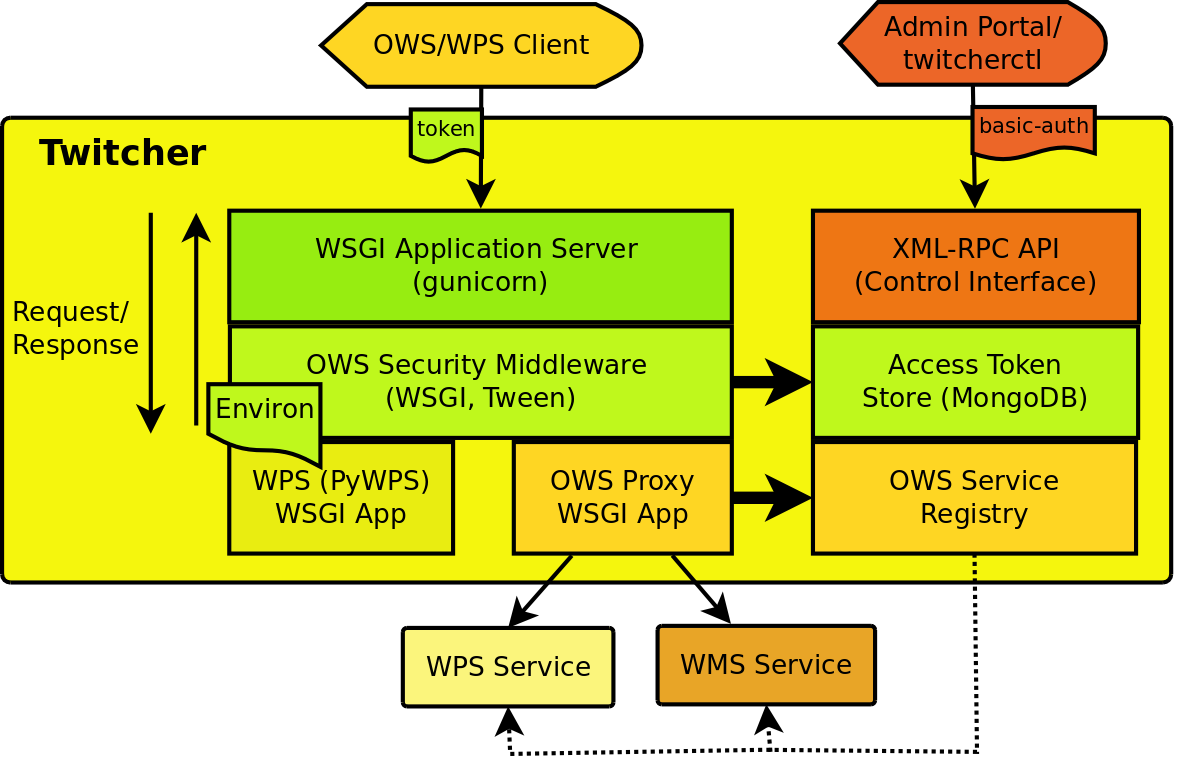
\includegraphics[height=5.85cm]{images/twitcher}
  \end{figure}

\end{frame}

\end{document}
